\section{Purpose}
The Bloch equations provide a mathematical framework for characterizing the evolution of the magnetization over time. These equations describe the magnetization $B=(M_x, M_y, M_z)$ in terms of time $t$, the relaxation time $T_1$, $T_2$, and the external magnetic field $B$ and can be solved analytically with an explicitly defined pulse sequence. Though the Bloch equations play a crucial role in various applications of magnetic resonance imaging (MRI) and allow us to understand the behavior of the magnetization and obtain images, due to the nonlinear dynamics system they described, it is difficult to utilize the extensive parameters space in the pulse sequence to optimize our signal, especially when considering some physiological or technical limitations.
\\\\
Reinforcement Learning shows its huge potential in dealing with dynamic environments, particularly in areas such as gaming and autonomous systems (Chess and Go). It is a type of machine learning where an agent learns to make decisions by performing actions in an environment to maximize a reward signal. This approach allows the agent to learn from experience, adjusting its behavior over time to achieve the best results without knowing much about the action which have been used but simple rules.
\\\\
The main objective of this project is to optimizing MRI pulse sequence using Reinforcement Learning. Given a typical gradient-echo sequence-based signal, the goal is to design a new sequence that can produce an optimized signal under certain constraints including slew rate of a magnetization gradient field. A Python package will be released.

\section{Literature Review}

0038 presents a RL framework to solve the general design problem of pulse sequence. The target signal is obtained with a pre-defined pulse sequence and Bloch Equations under some constraints to meet experiment equipments and as showed in Figure.\ref{schematic}, the pulse sequence X(t) is generated by a agent from a distribution p(X). The distribution p(X) is modeled by a dependent Gaussian process. The interaction between action X(t) and environment is simulated by a Bayesian neural network f:X(t) -> y, where y is the score of the predicted signal compared with the target signal. To deal with the exploitation and exploration dilemma, the next set of pulse sequence $X^*$ is proposed by $p\left(f \mid y_t, X_{t+1}\right)$ by maximizing the acquisition function $u_t(X)$. They developed the MR physics simulator based on tool MRILAB. They performed the framework in 1-D experiments gradient echo with a fixed RF pulse, two simple constraints on $G_x$ is applied and gained a satisfied result. 0477 extended this framework to RF pulse design in 2-D experiments and showed the potentiality of the application of RL in pulse sequence design.

\section{Methodology}

Our method will mainly follow the idea of the last two articles. The detailed implementation of algorithm will based on the MRILAB. The simulation of Bloch Equation with explicit gradient sequence has already been implemented in Python. This project will focus on designing 2-D Gradient Echo and after carrying out the algorithm implementation of the basic model, we will pay more attention on optimizing the slew rate of gradient.

\section{Challenge}

The foreseeable challenges of this project can be divided into several parts.
\\\\
Though the basic mechanism in MRI with pulse sequence has been taught in the related course, there is still a lot of relevant research that needs to be done, most notably to explore the constraints of mechanical properties on sequence design, in terms of performance and efficiency, in a realistic environment. In the current study, the main focus is on how to evaluate the slew rate and the effect of the overlap of two gradients on the output signal.
\\\\
This project involves the knowledge of Reinforcement Learning and Bayesian Neural Network that I had not learned before, so understanding and implementing the algorithms will be another major part of this project. Additionally, as our algorithm will involve huge matrix multiplication, optimizing our algorithms to reduce the running time in an acceptable time with a limited computational resources should be considered.

\begin{figure}[ht]
    \centering
    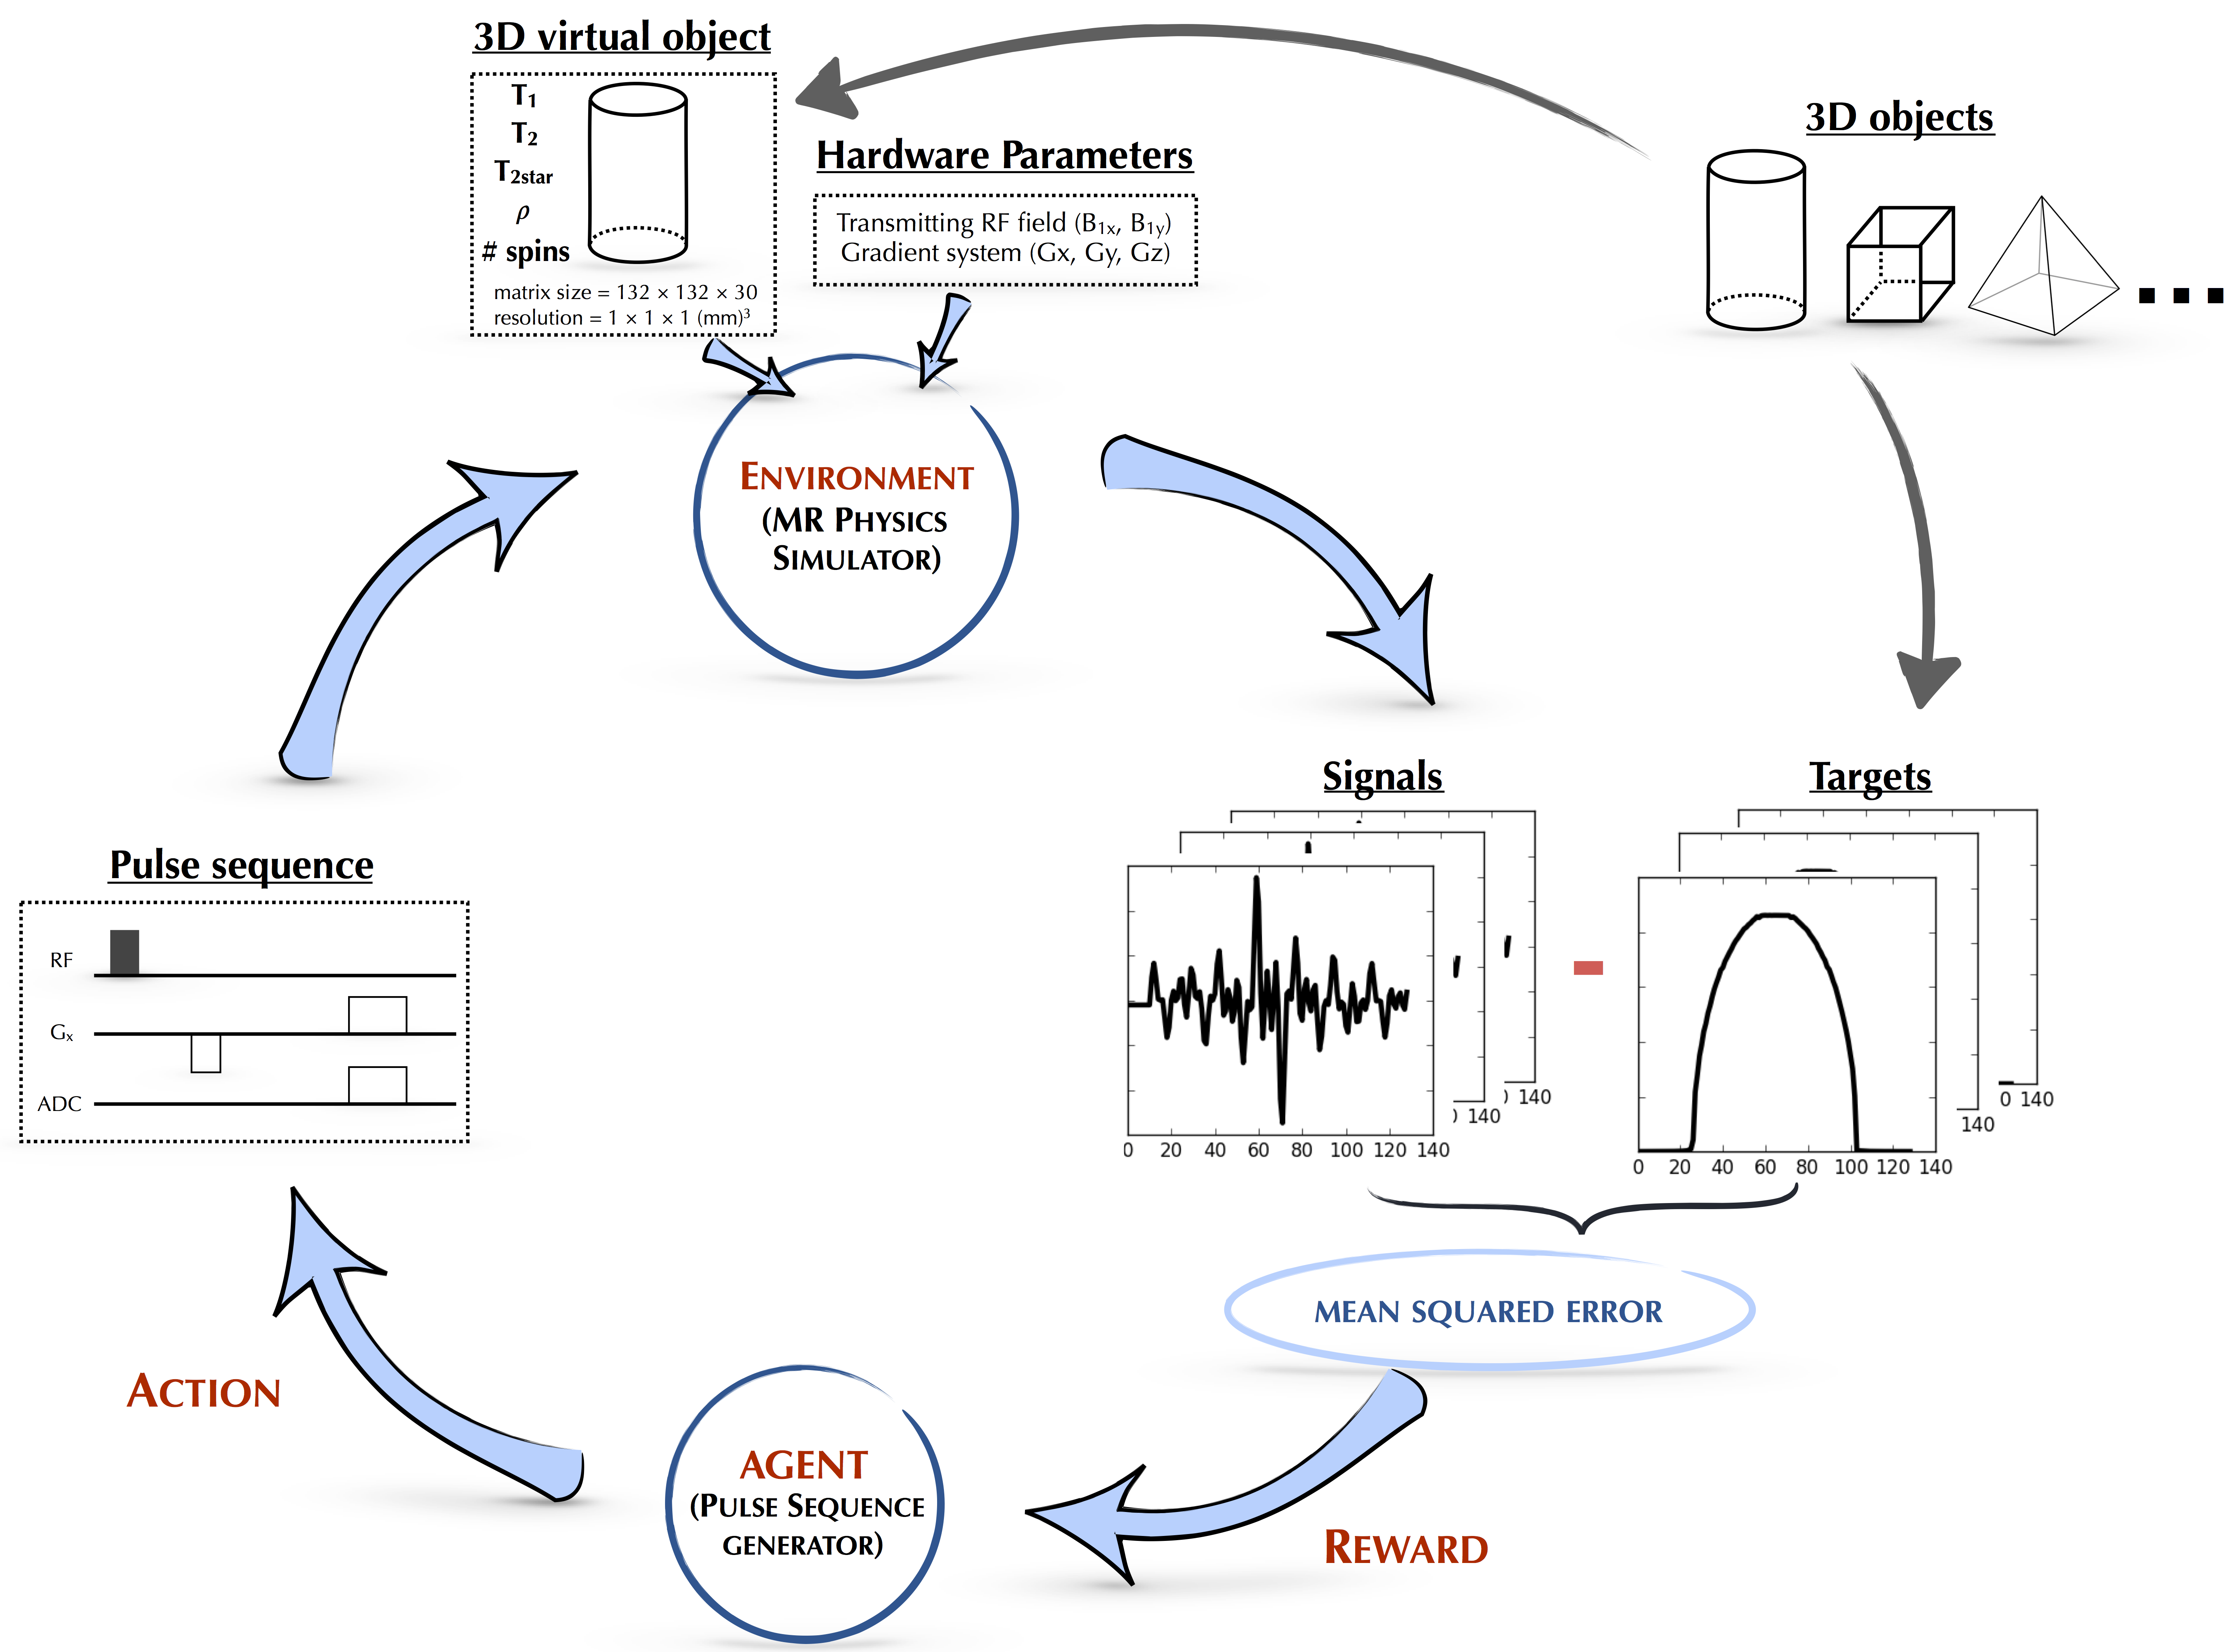
\includegraphics[scale=0.6]{schematic.png}
    \caption{title}
    \label{schematic}
\end{figure}

\section{Reference}
